\documentclass[tikz,border=4pt]{standalone}
\usepackage{amsmath,amssymb}
\usepackage[compat=1.1.0]{tikz-feynman}
\usetikzlibrary{arrows.meta,positioning,automata,shapes,shapes.misc,calc,decorations.pathmorphing,decorations.markings,angles,quotes,patterns,mindmap,matrix,knots,hobby,trees}
\tikzset{->-/.style={decoration={markings, mark=at position 0.5 with {\arrow{Stealth}}}, postaction={decorate}}}
\begin{document}
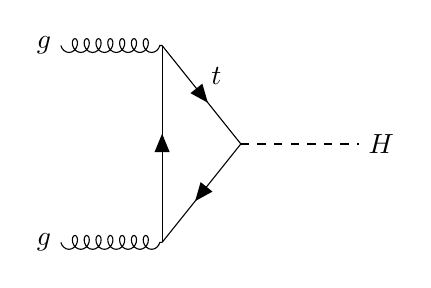
\begin{tikzpicture}
\begin{feynman}
\vertex (g1) {\(g\)}; \vertex [below=2.5cm of g1] (g2) {\(g\)};
\vertex [right=1.5cm of g1] (t1); \vertex [right=1.5cm of g2] (t2);
\vertex [below right=1.25cm and 2.5cm of g1] (t3); \vertex [right=1.5cm of t3] (h) {\(H\)};
\diagram* {
  (g1) -- [gluon] (t1), (g2) -- [gluon] (t2),
  (t1) -- [fermion, edge label=\(t\)] (t3) -- [fermion] (t2) -- [fermion] (t1),
  (t3) -- [scalar] (h),
};
\end{feynman}
\end{tikzpicture}
\end{document}
